\chapter{Introduction}
Accurate forecasting of time series data has been a topic of great interest, for its many different application, such as improving the quality of decision-making processes in strategic sectors of governments and enterprises. As a result, over time many different models have been developed to achieve this goal. Statistical and Machine Learning (ML) methods have stood out in the area of time series forecasting in the course of the years. Traditional statistical linear methods, such as the ARIMA (Auto-Regressive Integrated Moving Average) model and its variants, have proven effective for capturing linear dependencies and seasonality in data. Such methods assume a linear correlation structure of time series patterns; therefore, these models may present reduced accuracy in forecasting real-world time series since these can present linear and nonlinear temporal patterns \cite{SANTOSJUNIOR2023119614}, \cite{kontopoulou2023review}. On the contrary, machine learning methods offer the flexibility to capture complex nonlinear patterns without relying on strict assumptions about the data's correlation structure, however, this models may not learn nonlinear and linear patterns equally due to misspecification of the parameters, which can lead to underfitting or overfitting. For this reason, many approaches in the literature have proposed hybrid models that combine the strengths of both statistical and machine learning methods to capture linear and nonlinear relationships in time series data \cite{zhang2003hybrid}, \cite{abraham2017hybrid}. One particularly promising approach discussed in the literature is \textbf{residual ensembling}, which involves modeling the linear and nonlinear patterns sequentially. The approach can be summarized in this way:
\begin{itemize}
    \item a classical linear model such as ARIMA is first applied to the time series to capture linear trends and seasonality
    \item the model’s predictions, denoted as $\hat{y}$ are then subtracted from the actual values $y$ to obtain the residuals, which should only contains the nonlinear patters of the data
    \item these residuals are then used as input to a machine learning model, which is designed to capture the remaining complex, nonlinear relationships
    \item the predictions of the linear model and of the ML model are then combined to get a single prediction.
\end{itemize}
The objective of the thesis is to propose an ensemble of models that combines the strengths of classical statistical models to capture linear dependencies with machine learning models and deep learning models to capture nonlinear dependencies. This methodology is visually represented in Figure \ref{fig: Residual learning}, taken from \cite{SANTOSJUNIOR2023119614}:
\begin{figure}[H]
    \centering
    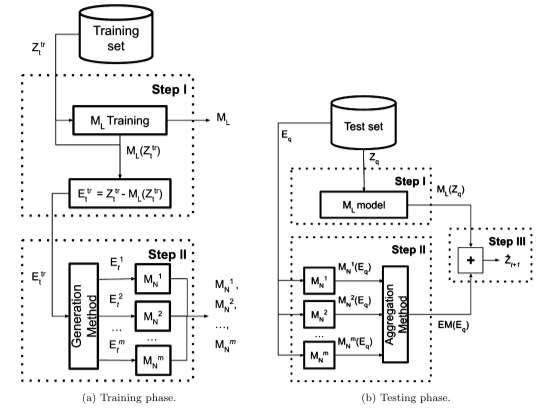
\includegraphics[width=0.50\textwidth]{Machine_learning_thesis/Images/residual learning.png}
    \caption{Residual learnign process.} 
    \label{fig: Residual learning}
\end{figure} 
Recent literature indicates that on tabular data classical machine learning approaches often outperforms deep learning methods, in particular tree ensembles, such as XGBoost can outperforms state-of-the-art DNN models by efficiently feature-engineering the input and output structures \cite{elsayed2021do}, \cite{grinsztajn2022why}, \cite{shwartz2022tabular}. Consequently, this thesis aims to model nonlinear relationship combining tree ensemble models with deep learning models to obtain a more accurate result, as demonstrated by the following study \cite {shwartz2022tabular}. Finally, in order to combine the prediction of each base model, multiple ensemble techniques have been proposed, but the one that seems more promising and that will be used in this thesis, in order to achieve a state-of-the-art ensemble model, is named \textbf{Arbitrated Dynamic Ensemble}, proposed in following article \cite{castro2023arbitrated}, which enables to dynamically adjust the weighting of each model’s contribution based on recent patterns in the data, making the ensemble more responsive to changing trends. It consists in a meta-learner approach, designed to predict how accurate the base models will predict based on the most recent data points, which then allows to predict which model is more likely to predict well in that context, adjusting the weights as a consequence. The structure can be sumarize by the image provided by the author of the paper: 
\begin{figure}[H]
    \centering
    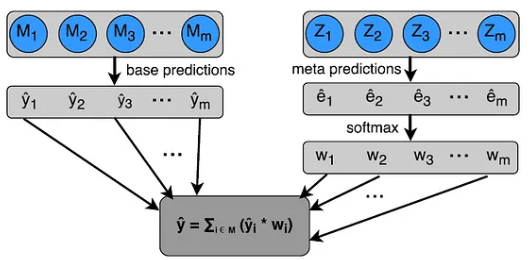
\includegraphics[width=0.50\textwidth]{Machine_learning_thesis/Images/Arbitrated Dynamic Ensemble.png}
    \caption{Arbitrated Dynamic Ensemble process.} 
    \label{fig: Arbitrated Dynamic Ensemble}
\end{figure} 
The final prediction will then be obtained as a weighted average of the weights dynamically computed: 
\[
\hat{y} = \sum_{i \in 1} \hat{y_i} w_i
\]



\section{Structure of the Thesis }
